% This is "sig-alternate.tex" V2.0 May 2012
% This file should be compiled with V2.5 of "sig-alternate.cls" May 2012
%
% This example file demonstrates the use of the 'sig-alternate.cls'
% V2.5 LaTeX2e document class file. It is for those submitting
% articles to ACM Conference Proceedings WHO DO NOT WISH TO
% STRICTLY ADHERE TO THE SIGS (PUBS-BOARD-ENDORSED) STYLE.
% The 'sig-alternate.cls' file will produce a similar-looking,
% albeit, 'tighter' paper resulting in, invariably, fewer pages.
%
% ----------------------------------------------------------------------------------------------------------------
% This .tex file (and associated .cls V2.5) produces:
%       1) The Permission Statement
%       2) The Conference (location) Info information
%       3) The Copyright Line with ACM data
%       4) NO page numbers
%
% as against the acm_proc_article-sp.cls file which
% DOES NOT produce 1) thru' 3) above.
%
% Using 'sig-alternate.cls' you have control, however, from within
% the source .tex file, over both the CopyrightYear
% (defaulted to 200X) and the ACM Copyright Data
% (defaulted to X-XXXXX-XX-X/XX/XX).
% e.g.
% \CopyrightYear{2007} will cause 2007 to appear in the copyright line.
% \crdata{0-12345-67-8/90/12} will cause 0-12345-67-8/90/12 to appear in the copyright line.
%
% ---------------------------------------------------------------------------------------------------------------
% This .tex source is an example which *does* use
% the .bib file (from which the .bbl file % is produced).
% REMEMBER HOWEVER: After having produced the .bbl file,
% and prior to final submission, you *NEED* to 'insert'
% your .bbl file into your source .tex file so as to provide
% ONE 'self-contained' source file.
%
% ================= IF YOU HAVE QUESTIONS =======================
% Questions regarding the SIGS styles, SIGS policies and
% procedures, Conferences etc. should be sent to
% Adrienne Griscti (griscti@acm.org)
%
% Technical questions _only_ to
% Gerald Murray (murray@hq.acm.org)
% ===============================================================
%
% For tracking purposes - this is V2.0 - May 2012

\documentclass{sig-alternate}

\usepackage{graphicx,subfigure,color}
\usepackage[usenames,dvipsnames]{xcolor}
\usepackage[moderate]{savetrees}
\usepackage{url}
\usepackage[font=bf]{caption}
\usepackage{natbib}


% Set letter paper size:
\setlength{\paperheight}{11in}
\setlength{\paperwidth}{8.5in}
\usepackage[
  pass,% keep layout unchanged 
  % showframe,% show the layout
]{geometry}

\newcommand{\fig}[3][1.0]{
\begin{figure}[tbp]
\begin{center}
\includegraphics[width=#1\columnwidth]{figs/#2}
\protect\caption{#3}
\label{fig:#2}
\end{center}
\end{figure}
}

\newcommand{\widefig}[3][0.9]{
\begin{figure*}[htbp]
\begin{center}
\includegraphics[width=#1\textwidth]{figs/#2}
\protect\caption{#3}
\label{fig:#2}
\end{center}
\end{figure*}
}

\setlength{\belowcaptionskip}{-10pt}

\newcommand{\comment}[1]{\textbf{\color{green}((#1))}}
\newcommand{\todo}[1]{\textbf{\color{red}TODO: #1}}
\newcommand{\stag}[1]{\textbf{#1}}
%\newcommand{\example}[2]{\begin{quote}\hspace{-6ex}(R#1) \hspace{2ex} #2 \end{quote}}


\newcommand{\example}[2]{% 

\vspace{0.10cm}

\hspace{-3.9ex} \begin{tabular}{ p{0.6cm} p{7.15cm} }
    {\it \small (R#1)} & #2 \\
\end{tabular}%
\vspace{0.10cm}

}


\begin{document}

%
% --- Author Metadata here ---
\conferenceinfo{WWW2015}{Florence, Italy}
%\CopyrightYear{2007} % Allows default copyright year (20XX) to be over-ridden - IF NEED BE.
%\crdata{0-12345-67-8/90/01}  % Allows default copyright data (0-89791-88-6/97/05) to be over-ridden - IF NEED BE.
% --- End of Author Metadata ---

% \title{I Once was a Turnip: A Survey of Self-Curation, Deception and Privacy Concerns Online}
\title{Self Curation, Social Partitioning, Escaping from Prejudice and Harassment: the Many Dimensions of Lying Online}

% \subtitle{[Extended Abstract]
%\titlenote{A full version of this paper is available as
%\textit{Author's Guide to Preparing ACM SIG Proceedings Using
%\LaTeX$2_\epsilon$\ and BibTeX} at
%\texttt{www.acm.org/eaddress.htm}}}
%
% You need the command \numberofauthors to handle the 'placement
% and alignment' of the authors beneath the title.
%
% For aesthetic reasons, we recommend 'three authors at a time'
% i.e. three 'name/affiliation blocks' be placed beneath the title.
%
% NOTE: You are NOT restricted in how many 'rows' of
% "name/affiliations" may appear. We just ask that you restrict
% the number of 'columns' to three.
%
% Because of the available 'opening page real-estate'
% we ask you to refrain from putting more than six authors
% (two rows with three columns) beneath the article title.
% More than six makes the first-page appear very cluttered indeed.
%
% Use the \alignauthor commands to handle the names
% and affiliations for an 'aesthetic maximum' of six authors.
% Add names, affiliations, addresses for
% the seventh etc. author(s) as the argument for the
% \additionalauthors command.
% These 'additional authors' will be output/set for you
% without further effort on your part as the last section in
% the body of your article BEFORE References or any Appendices.

\numberofauthors{5} %  in this sample file, there are a *total*
% of EIGHT authors. SIX appear on the 'first-page' (for formatting
% reasons) and the remaining two appear in the \additionalauthors section.
%
% You can go ahead and credit any number of authors here,
% e.g. one 'row of three' or two rows (consisting of one row of three
% and a second row of one, two or three).

% The command \alignauthor (no curly braces needed) should
% precede each author name, affiliation/snail-mail address and
% e-mail address. Additionally, tag each line of
% affiliation/address with \affaddr, and tag the
% e-mail address with \email.
% 1st. author
% all the authors: eMax, DMR, Amy, DS, Nigel
\author{
\alignauthor Max Van Kleek\\
        \affaddr{Web and Internet Science}\\
        \affaddr{University of Southampton, UK}\\
        \email{emax@ecs.soton.ac.uk}
% 2nd. author
\alignauthor Dave Murray-Rust\\
        \affaddr{School of Informatics}\\
        \affaddr{University of Edinburgh, UK}\\
        \email{d.murray-rust@ed.ac.uk} 
\alignauthor Amy Guy\\
        \affaddr{School of Informatics}\\
        \affaddr{University of Edinburgh, UK}\\
        \email{Amy.Guy@ed.ac.uk}
\and  % use '\and' if you need 'another row' of author names
% 4th. author
\alignauthor Daniel A. Smith\\
        \affaddr{Web and Internet Science}\\
        \affaddr{University of Southampton, UK}\\
        \email{ds@ecs.soton.ac.uk}
% 5th. author
\alignauthor Nigel R. Shadbolt\\
        \affaddr{Web and Internet Science}\\
        \affaddr{University of Southampton, UK}\\
        \email{nrs@ecs.soton.ac.uk}
}
\maketitle


\begin{abstract}
% is this ok? => [ yes (tick) ] [ no ]
% do you want me to kill HARASSMENT hahah
% ;) mostly for sentence structure... 
% how about if we rotate
% flip it and reverse it! betar?
% happy happy joy joy
% do we want truly in first clause? Helps readability

Portraying matters as other than they truly are is an important part of everyday human communication. In this paper, we use a survey to examine ways in which people fabricate, omit or alter the truth online. Many reasons are found, including creative expression, hiding sensitive information, role-playing, and avoiding harassment or discrimination. The results suggest lying is often used for benign purposes, and we conclude that its use may be essential to maintaining a humane online society.

% Portraying matters as other than 
% %``the whole and honest truth'' 
% they are
% is an important part of everyday human communication.
% %, both on and offline.
% In this paper, we use a survey to examine the ways in which people fabricate, omit or alter the truth online. Many reasons are found, including creative expression, hiding sensitive information, avoiding discrimination, role-playing and fitting in. The results suggest lying is often benign, and conclude that its use may be essential to maintaining a humane online society.
\end{abstract}

% Dave's epic magnum opus here :P
% \begin{abstract}
% Portraying matters as other than they truly are is an important part
% of communication for many reasons. As well as malicious deception, white lies and butler
% lies are used to smooth the process of communication or protect people
% from parts of reality. The choice of which parts of ourselves we
% present, and how, is a fundamental part of the construction of human
% identity. It may be necessary to hide certain aspects for fear of
% stigmatisation, or to maintain a separation between professional and
% personal contexts. The adoption of personas can
% be used to role-play alternative viewpoints, escape discrimination or
% for creative purposes.

% The increasing pervasiveness of personal information online threatens
% this ability; the \emph{context collapse} due to the increasing
% integration and permanence of data reduces peoples choice of how they
% present in and navigate through the digital landscape.

% In this paper we present the results of a survey of both the manner
% and reasoning for presenting mistruths, omissions and fictions on
% online social networks. Multiple reasons for lying, omission and
% fiction are found in the responses, including: creating personas for
% fun or artistic reasons; hiding sensitive information to avoid
% harassment or stalking; role-playing to understand other's viewpoints
% or avoid discrimination; fitting in with social norms; and a sense
% that personal information is not relevant or should be kept under
% control. This is contextualised with demographic information about
% attitudes to privacy, evaluations of friends behaviour and which
% social networks are used.

% The results indicate that most people lie and withold information for
% benign purposes: self protection, choice of presentation, insulating
% others or creative reasons. We argue that preservation of this
% facility is essential to maintaining a humane online society.
% \end{abstract}

% A category with the (minimum) three required fields
\category{H.4}{Information Systems Applications}{Miscellaneous}
\category{J.4}{Social and Behavioral Sciences}{Sociology}
%A category including the fourth, optional field follows...
%\category{D.2.8}{Software Engineering}{Metrics}[complexity measures, performance measures]

% \terms{}

\keywords{Lying online, privacy, digital identity, online communities}

\section{Introduction}

% , and has remained the subject of philosophical and theological discussion and debate for centuries~\cite{sanford}

% spectrum ranging from the ordinary connotations associated with deception as a deliberate attempt
% to mislead others to a much larger class of activities that involve portraying information in a way 
% that parts from the full and open representation of understood reality.

Lying and other forms of deception are as fundamental to human interaction as discourse itself, amounting to as much as a third of interpersonal communications by some accounts~\cite{depaulo1996lying,bok2011lying}.  By deception, we refer to not only the standard connotation of a deliberate attempt to mislead others, but to a much larger class of activities characterised as ``any conveyance of information that does not reflect the entirety of known truth''~\cite{camden1984white}.  Deliberately included in such a definition is the construction of personas or identities meant to represent one's self with attributes different from one's own. 

The benefit of studying such deception in the context of social interaction is that it illuminates the ways that people cope with the complexities of the social demands placed on them, within the contexts where they live and work~\cite{camden1984white}.  
People conduct their interactions and curate their identities across a large number of online spaces, whilst attempting to maintain their privacy, reputation and roles throughout. Deception is a tool used to cope with this complexity, and a lens through which their difficulties and needs can be observered~\cite{hancock2007digital, Burgoon:2003:TDM:820748.821362}.  

Understanding the use of lying and deception online is important to developing and understanding the Web, because new social situations and their attendant complexities are created by the affordances of the technologies used as the channels for social interaction \cite{hancock2004deception}.  Technologies that provide new means of social interaction, whether simply a new mobile chat app or a new communications capability entirely, can have unanticipated consequences.   For example, the immediacy and ubiquity of wireless communications technology is thought to have made commonplace the use of \emph{butler lies}, which are small lies invoked to avoid or take leave of interaction \cite{hancock2009butler} without causing offence.  

In this paper, we present a summary of a survey-based study in which we sought to characterise the spectrum of lying and deception practices routinely used online. We are concerned with the ways in which people carry out the production of mistruth, and the manner in which it varies across different social media channels.
We are interested in the intent behind the deception, but we do not examine the moral or ethical dimensions of such practices, as these can be highly subjective and grounded in particular personal philosophies.
We find that while there are a wide range of reasons people use deception or identity protection online, few reasons for doing so are malicious (or comprised of ``dark lies''); in fact, a majority of the reasons pertain to impression management, conflict avoidance, and in order to fit in to groups.

In the following sections, we first briefly review the literature on online deception and lying. Second, we briefly describe our methodology and present our results. In the final section, we discuss the implications of our findings 
for the development of the Web,
in particular within the context of the increasing centralisation of social networks and rise of web identity assurance providers.

\section{Background}

% In this section we briefly discuss three sets of related work; first, we discuss a few key studies from social psychology pertaining to lying and deception, followed, second, by an overview of the much smaller literature on deception through computer-mediated communications (CMC) channels, folllwed, in turn, by a description of studies on identity curation, pseudonymous and privacy-preserving behaviours primarily by teens ans other social media users online. 
 
While several detailed frameworks for characterising different kinds of deception have been proposed in the social psychology literature, the most common approach divides lies into two general classes: \emph{everyday lies} of
``little consequence or regret'', and \emph{serious lies}, used typically to ``hide transgressions'', ranging from misdeeds to betrayals of trust~\cite{depaulo1996lying}. These notions correspond to the common distinction between harmless or beneficial \emph{white lies}, 
and socially or morally reproachable lies. A third category of \emph{grey lies} exists in between~\cite{camden1984white}.
%\todo{Can't find this in the 96 paper, closest I can find is in the 94 one, but the
%categories are different:On the strategic side,
%deceivers are likely to engage in information management, image management,
%and behavior management. }
In order to characterise the motivations behind lying, Buller and Burgoon derive three categories: \emph{instrumental}, \emph{relational}, pertaining to interpersonal relations, and \emph{identity-related}, pertaining to reputation management~\cite{buller1996testing}. 

A number of studies have compared online to offline lying practices. When looking at the \emph{richness} of communication environments --- the amount and immediacy of feedback for participants --- two competing theories arise. \emph{Media richness theory} postulates that lying is more likely in rich environments, while \emph{social distance theory} predicts more lying in impoverished settings, with fewer social cues, such as via e-mail.
Hancock et al.~\cite{hancock2004deception} analyse this competition, and  find support for the latter in their experiments.  
Belkin et al. compared lying in e-mail to paper, finding that people were likely to lie on e-mail signficantly more than in personal letters~\cite{naquin2010finer}.  

Sherry Turkle's seminal work on early digital spaces, \emph{Life on the Screen}~\cite{turkle2011life}, discusses the ways in which identity construction is a creative act, and linked to self development.
%\todo{Maybe misrepresenting, haven't read it DMR}
This desire to choose how one presents has been confirmed by many studies of online behaviour.
For example, the frequency with which gamers assume the opposite gender in online play~\cite{hussain2008gender,potts2014love,van2008theorizing}, assume widely different appearances in online virtual environments and massively multiplayer games~\cite{yee2009proteus}, falsify age, height, weight and appearances in online dating sites~\cite{Hancock:2007:TLO:1240624.1240697,JCC4:JCC420}, and experiment with self-representation in online chat and discussion spaces~\cite{donath1999identity,whitty2002liar,whitty2001age}.

Most similar to the work presented in this paper, Caspi et al.~\cite{caspi2006online} conducted a Web survey of Israeli internet users and found that, although a majority of participants believed that deception on the Internet was widespread, only a third ever reported deceiving others online themselves.  Instead of open-ended responses, however their survey asked participants to select among a fixed set of possible personal attributes (age, sex, marital status, height, weight, etc.) and the reasons for doing so. Our study complements theirs by providing a significantly larger set of ways people use deception, omission and false attributes, and justifications for doing each. % \todo{Do we?} We compare our results to theirs in Discussion.

\section{Method}


We elicited responses via a multi-page web-based survey, comprising 12 sets of questions including 1 set of demographic questions, and 8 open-answer free responses. In this paper, we focus on a subset of the questionnaire as shown in Figure \ref{fig:questionnaire}.  Participant recruitment was done in person at two events in London, at \emph{ComicCon} and the \emph{WebWeWant Festival}, and on-line via Twitter and Facebook.  In person, we distributed fliers containing the URL to the survey, and posted the URL on visible locations where permitted.  
% Two popular Internet celebrities, @TheTomSka and @DameWendyDBE helped by posting a link to the survey on their Twitter feeds.

% \begin{figure}[t!]
%     \begin{tabular}{ l p{7cm} }
%     \small
%       Q1 & How often do you use each social media platform? \\
%       Q2 & How concerned are you about your privacy online? \\
%       Q3 & Privacy: from whom/what are you most concerned? \\
%       Q4* & Have you ever told lies / ``untruths'' online? Why? \\
%       Q5* & Do you use any pseudonyms online? Why? \\
%       Q6* & Have you ever deleted anything you posted online? \\
%       Q7* & Have you experienced privacy violations online?  \\
%       Q8-11* & Foursquare, YouTube, Tumblr, Twitter \\
%       Q12-13 & General Demographic questions
%     \end{tabular}
%     \caption{%
%     	Questionnaire structure, with starred questions corresponding to free response answers. We focus on Q4-7 in this paper.
%      }%
%   \label{fig:questionnaire}
% \end{figure}
\begin{figure}[tbp]
    \begin{tabular}{ l | p{7cm} }
    \small
      {\bf Q4a*} & Have you ever told lies / ``untruths'' online? Why? \\
      {\bf Q4b} & How often do you tell lies / ``untruths'' on social media? \\
      {\bf Q4c} & How often do you think your friends lie on social media compared to you? \\      
      {\bf Q5a*} & Do you use any pseudonyms online? Why? \\
      {\bf Q5b*} & Have you created any fictional personas? Why?
    \end{tabular}
    \caption{%
    	List of questions corresponding to subset of survey discussed in this paper; questions with stars indicate free response; the rest are 5-level Likert responses. 
     }%
   \label{fig:questionnaire}
   \vspace{0.25cm}
\end{figure}




Analysis of free-response questions was done using a \emph{grounded theory}~\cite{strauss1990basics} approach; themes were identified across responses through a process starting with open coding process by each of three researchers separately, followed by a discussion process where themes were refined and combined. Multiple themes were permitted per entry. Once consensus was achieved on themes, all responses for a given question were re-coded against the final set.

\section{Results}

Out of the $N=500$ survey responses, 39\% ($N=198$) provided a gender; 50.2\% responded female, 49.8\% male, and 1\% transgender.  With respect to age, 59\% responded, 91\% were between 18--25, 7\% between 26--35, and 2\% 36+.  The age distribution skew was likely the result of the young audiences at the two festivals; we discuss the potential implications of this distribution at the end of the paper.

% max commented this out since it's not so relevant > 
%Nearly all respondents were active social media users, although use of particular platforms varied significantly.  Figure \ref{fig:socialmedia} shows the self-reported Likert scores per platform for 6 social media platforms. The popularity of YouTube and Twitter for respondents was likely influenced by the method of recruitment (via Twitter), and the fact that one of the popular Twitter users who disseminated news of the survey is a popular YouTuber.  
% \begin{figure}[t!]
%  	  \begin{center}
%         \subfigure[Facebook]{%
%             \label{fig:fb}
%             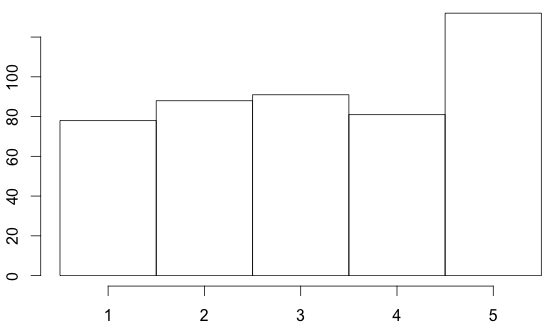
\includegraphics[width=0.24\textwidth]{figs/q1-fb}
%         }%
%         \subfigure[Twitter]{%
%           \label{fig:twitter}
%           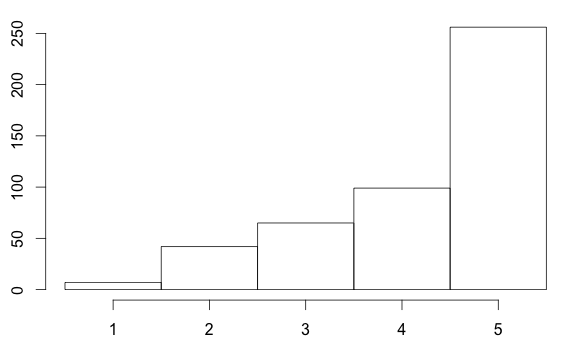
\includegraphics[width=0.24\textwidth]{figs/q1-twitter}
%         }\\ %  ------- End of the first row ----------------------%
%         \subfigure[YouTube]{%
%             \label{fig:youtube}
%             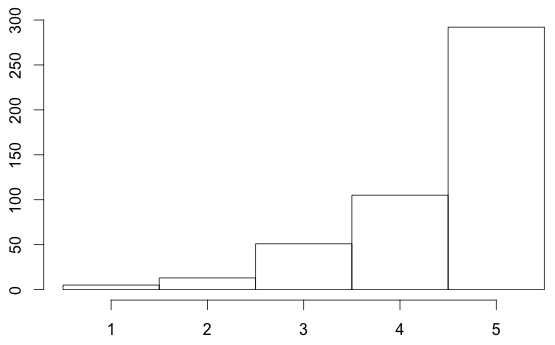
\includegraphics[width=0.24\textwidth]{figs/q1-youtube}
%         }%
%         \subfigure[Tumblr]{%
%             \label{fig:tumblr}
%             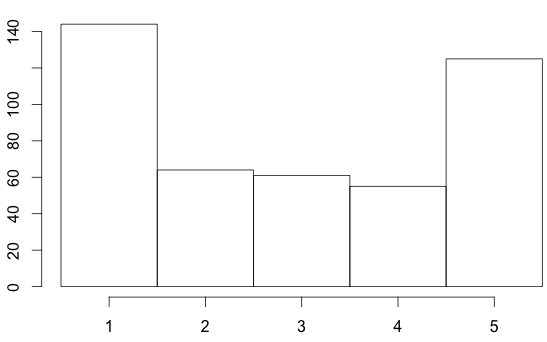
\includegraphics[width=0.24\textwidth]{figs/q1-tumblr}
%         }\\ %
%         \subfigure[Instagram]{%
%             \label{fig:instagram}
%             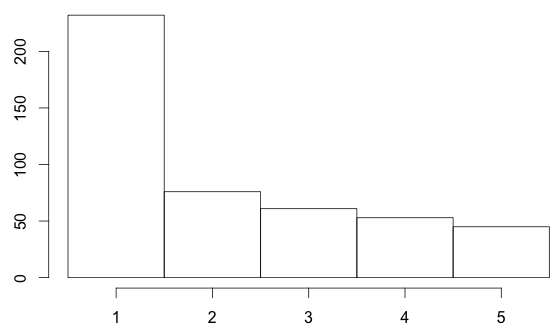
\includegraphics[width=0.24\textwidth]{figs/q1-instagram}
%         }%
%         \subfigure[Vine]{%
%             \label{fig:vine}
%             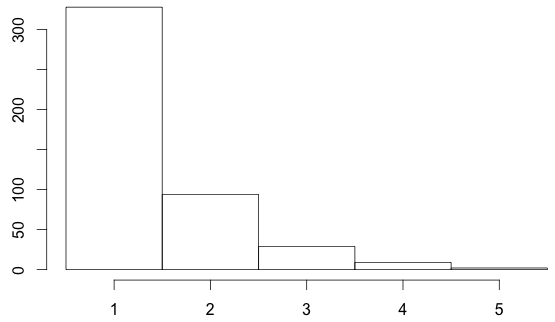
\includegraphics[width=0.24\textwidth]{figs/q1-vine}
%         }\\ %        
%     \end{center}
%     \caption{%
%     	Self-reported use of social media, from \emph{1=Never} to \emph{5=Often} times a day. Medians: $facebook=3$, $twitter=5$, $YouTube=5$, $Tumblr=3$, $Instagram=2$, $Vine=1$
%      }%
%   \label{fig:socialmedia}
% \end{figure}

\subsection{Self-reported frequency of deception/lying}

In terms of frequency of lying, $77\%$ of participants ($N=387$) responded to \emph{Q4b}, \emph{How often do you lie on social media?} 
% don't think we need it as it's on the fig. Also text in math mode? :P
% can change graph to 1 (never) if you're worred.
%on a scale from $1=Never$ to $5=Often$;
the distribution of answers is is displayed in Figure \ref{fig:freqlying}a.  The median response was 2, with a majority ($N=330$, $85\%$) of responses answering either a 1 or 2. % Slightly more than people answering never were people answering a '2'

% The scale is a bit dicey here - it can't really be the same scale, as one is
Question 4c asked \emph{How often do you think your friends lie on social media compared to you?}, 
and $77\%$ ($N=386$) again responded overall (Figure \ref{fig:freqlying}b). 
%received a much more even distribution around the value of $3$, as visible in Figure \ref{fig:freqlying}b, 
% can't have a key component of a sentence in parens - need either the number
% or percent in main flow.
% Missing the N value for 3 here (previously it was N=3, which I don't think is right. correct, good catch ;)
The median value was $3$, with ($N=87$, $22\%$) responding with a value that their friends lie less than they do (e.g. $1$ or $2$), while ($N=119$, $30\%$) responded that their friends lie more (e.g. $4$ or $5$).


\begin{figure}[tbp]
 	\begin{center}
 	    % Trying new diagram - ditch it if you like, but it's a 
 	    % bit smaller and more consistent
        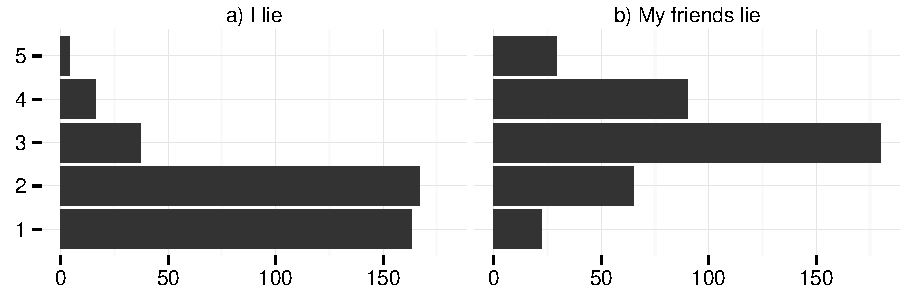
\includegraphics[width=1.0\columnwidth]{figs/q4cgraph}
        %\subfigure{%
            %\label{fig:lf}
%            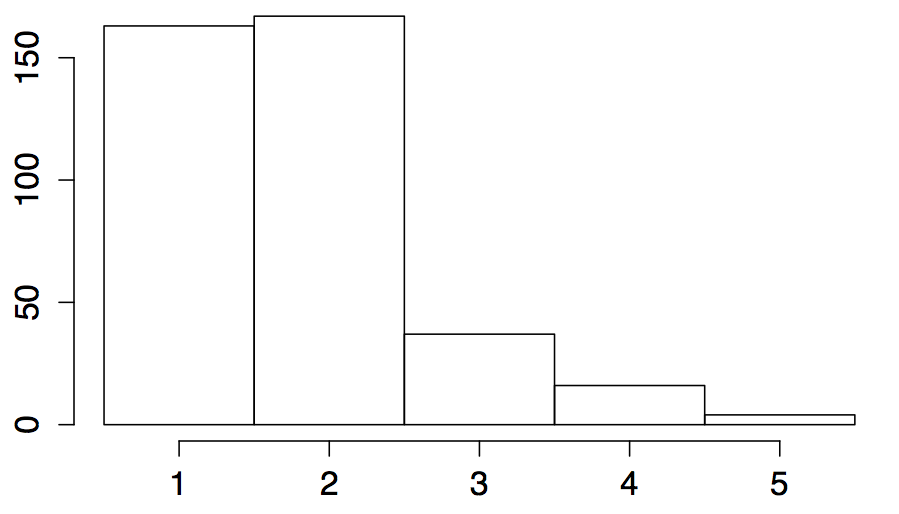
\includegraphics[width=0.23\textwidth]{figs/q4lies}
        %}%
%        \subfigure{%
           %\label{fig:lff}
%           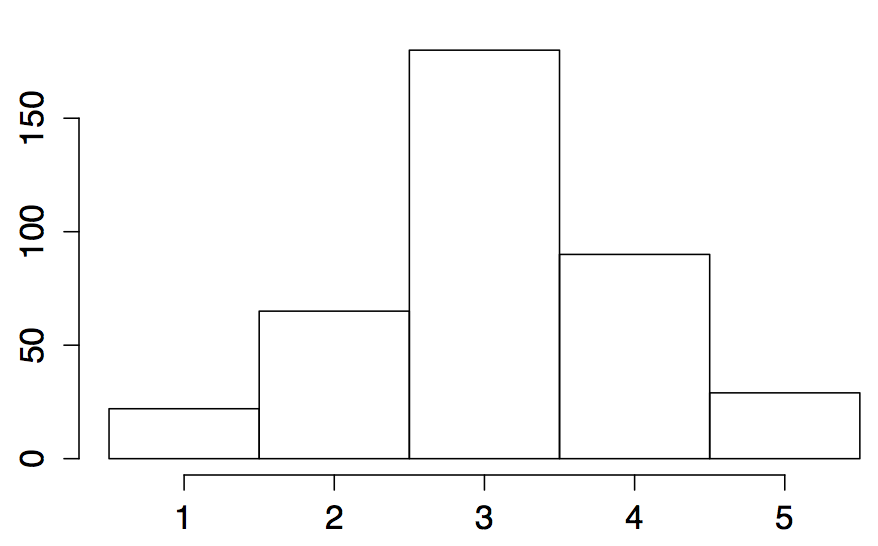
\includegraphics[width=0.23\textwidth]{figs/q4liesfriends}
        %} %  ------- End of the first row ----------------------%
    \end{center}
    \caption{%
    Responses to \emph{Q4b} and \emph{Q4c} on Likert scales 
    a) \emph{How often do you tell lies or untruths on social media?} 
    (\emph{1=Never} to \emph{5=Often})
    b) \emph{How often do you think your friends lie on social media compared to you?}
    (\emph{1=Vastly less} to \emph{5=Vastly more}) 
     }%
   \label{fig:freqlying}
\end{figure}

\subsection{Reasons for Deception} \label{sec:reasons}

A total of $N=134$ responses were received for $q4$, which asked people to explain whether they remembered telling lies (or ``untruths'') online and to explain the circumstances.  Out of the total respondents a quarter ($N=34$, 25\%) answered that they had or did not lie or use any form of deception online. The rest of the respondents admitted to having, or performing some form of deception regularly.  Thematic coding of the remainder of the responses revealed $10$ themes, listed in Table \ref{fig:q4themes}, plus an extra for \emph{yes}, a category standing for responses admitting participating in deception with no explanation, and \emph{no} for responses that denied using deception on social media. Tagging each response with the themes yielded $M=1.08$ themes per category, with a minimum of 1 and maximum of 3 ($\sigma^2=0.3$).  The number of responses falling into each of the themes is visible in Figure \ref{fig:q4frequency} (again, a response may be assigned to more than one theme).

% \color{red, green, orange, yellow, magenta, cyan, blue, sepai, purple, gray}
\begin{figure}[tbp]
        \small
    \begin{tabular}{  r | p{5.5cm}  }
        \textbf{playup} & To exaggerate, fabricate, falsify, or embellish to enhance image \\
        \textbf{playdown} & To make seem less significant, e.g. stop people from worrying \\
        \textbf{conform} & To omit, distort or falsify to blend in with others  \\
        \textbf{mitigate} & To escape or end awkward or difficult social interactions,  seem polite, including butler lies \\
        \textbf{creative} & ``Just to mess with people'', for fun/entertainment/humour/out of boredom. \\
        \textbf{explore} & To experiment with altering aspects of identity to explore effects on interactions \\
        \textbf{safety} & To protect self \\
        \textbf{soceng} & To trick people, falsely gaining trust to achieve some goal \\
        \textbf{privacy} & To preserve privacy or prevent identity linkage \\
        \textbf{coherence} & To backing up lies told elsewhere \\
        \textbf{no*} & Do not lie \\
        \textbf{yes*} & Do lie, but without explanation \\
    \end{tabular}
    \caption{\emph{Q4 Tags} --- List of themes and categories resulting from analysis of \emph{Question 4: Have you ever told ``untruths'' on social media, given fictitious info, omitted or distorted the truth online?}.} \label{fig:q4themes}
\end{figure}


% todo : can someone fill in 'foo' pls?
% N=35 because playup = playup*31, + (coherence; playup), + (playup; creative) + (playup; mitigate) + (privacy; playup; playdown)
The most prominent theme was \textbf{playup} (N=$35$), which corresponded to the rationale of wanting to be more appealing, interesting or attractive to others.  There were several subtypes of this activity, starting with simply falsifying personal attributes (height, weight, age) towards what s/he perceived would make him or her more attractive, to \emph{exaggerating} details of stories, to making things ``seem relatable''. Four mentioned aspects relating to making one's self seem popular or important by filling his or her social calendar to appear busy, while two discussed fabricating stories, such as of having met celebrities.  Contexts ranged from online dating to social interaction with strangers. 

%Less common, although present were responses about the entire fabrication or creation of fictional events and situations (3), while two respondents describing appropriation other people's content, including ``funny tweets'' and status posts, as if they had been their own.

Far less common ($N=9$, 7\%) was the opposite reason, in which participants reported deliberately distorting or omitting information in order to not \emph{attract} attention or in many cases to prevent disclosure of illness or situation to protect one's reputation.  This theme, coded as \textbf{playdown}, included the following responses:

\example{354}{Lied about my mental health countless times, denied depression and suicidal thoughts. }
\example{461}{I very selectively curate my online personae, particularly on Facebook, where I am careful to hide my mental illness, my frustrations, and my negative emotions.}
\example{49}{I tend to lie about how sick I am so people don't worry/employers don't get anxious.}


\fig{q4frequency}{\emph{Q4 Theme Counts} --- Raw counts of number of responses in each theme. The code `yes' indicates an affirmative response where no  justification was given. Responses which were unclear have been removed. Figure \ref{fig:q4themes} lists descriptions for each theme.}


The second most prominent theme after \textbf{playup} was \textbf{privacy}, a theme used to encompass a variety of privacy related concerns.  Respondents reported explicitly withholding information often, and, where information was required, providing false values about themselves.  The attributes most often mentioned were age ($N=17$), real name ($N=13$), physical location ($N=6$), gender ($N=3$) and birth date ($N=2$) to web sites that they did not trust.  Four mentioned that this in order to prevent identity linkage to their real-world identities, e.g.:
% \comment{Don't think this quote is quite about linkage across online services - it's more to the realworld}
\example{461}{On fetish sites, I will lie about my birthday (displacing my age by a few months to a year in the process) and my hometown, making my identity there harder to connect to my real identity.}

Others expressed that they adopted the strategy of falsifying attributes when social networks asked for information that were unnecessary, for example:

\example{500}{Whenever a social media asks me to provide personal details which are not directly necessary for them to deliver the service (e.g. Facebook asking for my workplace), I constantly feed them wrong information. First and foremost to stop them asking me for such information while at the same time keeping my personal data private.}

A different reason given for falsified attributes was coded as \textbf{conform}, when falsification was done in order to fit in, in particular to avoid harassment and discrimination.  Such behaviour including avoiding potential confrontation surrounding personal beliefs (pertaining to religion or politics), or to personal attributes including gender, age, race or sexual orientation.  One participant described her choice of declaring herself as male improved her position in debates online which were often predicated with \emph{ad feminam} attacks on her gender:

\example{301}{The major untruth I tell is pretending to be a man rather than a woman on YouTube - I know it's bad and not helping the cause, but I know that if I want to convince someone of a particular point, if I pretend to be a man my sayings won't be regarded through the bias of my gender, while if I say opinions (completely disconnected from gender issues) as a woman, it will probably be the 1st thing my opponents will use in a debate.}

Another set of responses ($N=7$) described the use of deception in order to deceive, trick or manipulate situations to the individual's advantage; such reasons were coded \textbf{soceng} because it reflected the common notion of ``social engineering''.  The most common example of this (5 out of 7) involved simply falsification of age in order to gain access to age-restricted content online. The remaining two pertained to falsification of academic credentials for jobs and posing as another person online and attempting to attract her partner's attentions as this fake identity in order to test her partner's loyalty.

A smaller category  ($N=6$) corresponded to deception or lies told for fun, humour, or ``just messing about''. The tag \textbf{creative} was used for this group, which included examples such as pretending to have a twin, pretending to have met someone famous, or permuting another person's words.  

Lies used to diffuse, or bring an end to, unwanted social situations we called \textbf{mitigate}.  This class ($N=7$) was a superset of butler lies, while butler lies serve primarily to terminate and divert unwanted social interactions, the lies in this category included those told to be polite, such as agreeing with a person to avoid an argument. Meanwhile, \textbf{safety} ($N=3$) corresponded to the responses describing omission or falsification to avoid compromising one's physical safety, or from potential litigation for potentially illegal activities.

Finally, the two smallest categories, \textbf{explore}, and \textbf{coherence} each had two responses.  The first, \textbf{explore}, pertained to responses that discussed experimenting with aspects of their identity, in particular to ``test the reactions of others'', a category corresponding to the tag \textbf{experiment} for $q5$, as described in the next section.  Meanwhile, \textbf{coherence} was the act of lying in order to maintain  consistency with other lies told elsewhere to prevent lies from being discovered. 

% Another respondent described initially falsifying his age due to his feeling insecure about being older than the group he was associating with:

% \begin{quote}
% (R48) I've misled by omission about my age as I'm a member of a 'fandom' where the base age is younger than myself and didn't want to make others uncomfortable. I've now 'fessed up as being a member for a while I started to realise there were others well over the average age too.
% \end{quote}

%\fig{q4q5}{Example figure showing results of tagging Q4 and Q5}
%\fig{q4}{Example figure showing results of tagging Q4}
%\begin{figure*}
%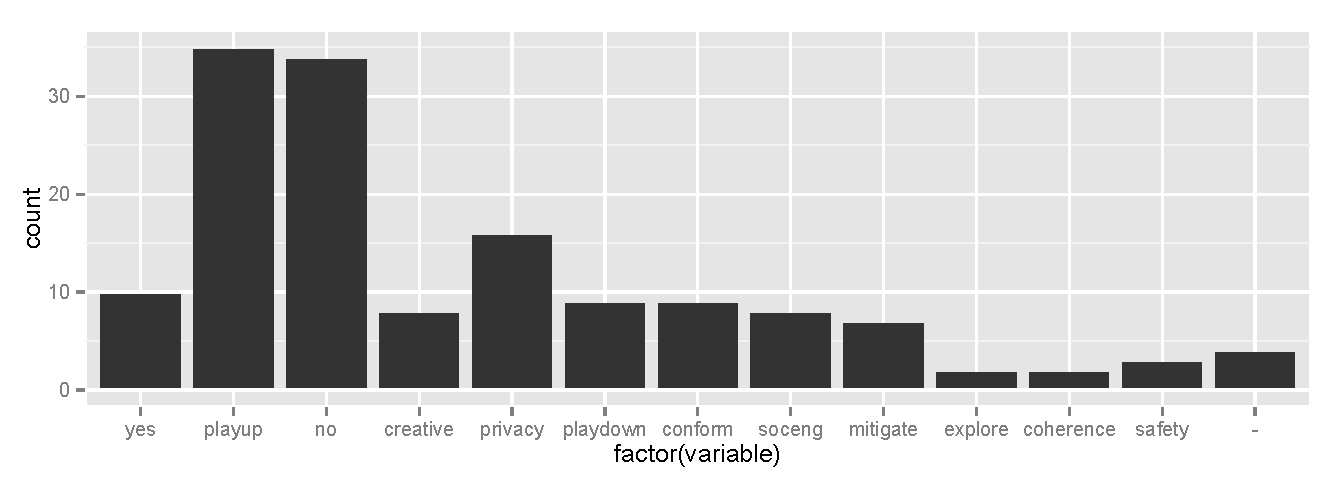
\includegraphics[width=1.0\textwidth]{figs/q4}
%\caption{Example figure showing results of tagging Q4}
%\label{q4}
%\end{figure*}



\subsection{Pseudonyms}
\label{sec:pseudonyms}

\begin{figure}[tbp]
    \small
    \begin{tabular}{ r | p{5.5cm} }
		{\bf bespoke} & Several online identities kept separate. \\
		{\bf character} & Role-playing an obviously fictional character. \\
		{\bf conform} & Conform to community norms, fit in with others. \\
		{\bf creative} & For entertainment or creative purposes. \\
		{\bf discoverability} & Use of a pseudonym to connect identities or be discoverable. \\
		{\bf discrimination} & Avoid being judged unfairly. \\
		{\bf disnomia} & Dislike real name. \\
		{\bf experiment} & Role-playing different real-world identities to experience the way they are treated, and/or trying to get someone else's viewpoints. \\
		{\bf expression} & Saying things without fear or repercussions. \\
		{\bf habit} & Force of habit. \\
		{\bf hide} & Hiding activities from everyone. \\
		{\bf identity} & Online identity more closely matching true self. \\
		{\bf intimate} & Posting intimate thoughts and feelings. \\
		{\bf no} & ``No'', with no reason given. \\
		{\bf nothide} & Use of a pseudonym, but not trying to hide one's identity. \\
		{\bf plus} & Mentioned the Google\texttt{+} ``real names'' policy. \\
		{\bf privacy} & General feeling of not wanting to reveal stuff. \\
		{\bf reuse} & Used a nickname or variation of offline names. \\
		{\bf safety} & Protection from other people. \\
		{\bf separation} & Separate concerns (professional, family, between friends).\\
		{\bf sex} & Anything about sex. \\
		{\bf soceng} & Tricking people or gaming the system e.g. falsely gaining trust, fake qualifications, circumventing age restrictions, using sockpuppets, and spam control. \\
		{\bf spy} & The system is spying on me, merging my accounts, and sharing data. \\
		{\bf yes} & ``Yes'', with no reason given. \\
		{\bf -} & Theme unclear from answer. \\
    \end{tabular}
        \caption{\emph{Q5 Tags} --- List of themes and categories resulting from analysis of \emph{Question 5a: Do you use pseudonyms on any social media platforms? Why do you do this? Do you try to hide your real name/identity?} and \emph{5b: Have you created any fictional personas (e.g., characters, \emph{alter-egos}) to use on social media?}
     }%
   \label{fig:q5themes}
\end{figure}

A total of $N=286$ responses were received for $q5a$, which 
asked for information about whether participants had used pseudonyms, and why. A group ($N=82,27\%$) claimed not to use pseudonyms online, and a further group ($N=5,2\%$) gave answers which were unclear.  This left 70\% of respondents claiming to have used an online pseudonym. 

The most common reason for pseudonym use was tagged as \stag{separation} ($N=63, 22\%$). This covers several different lines of division. The three most prevalent reasons were i) separating online and offline lives; ii) separating personal and professional identities; and iii) maintaining distinction between groups of friends or family:
\example{266}{\ldots It was mainly done to slightly separate my identity from reality and the internet.}
\example{79}{\ldots I also do not want future employers and such to be able to find all of my social media straight away and making judgements based on it.}
\example{150}{\ldots I used to have a nerdy YouTube channel which I did not want my peers finding out about, so almost all of my online activity connected to that was under a different (screen) name}


\fig{q5afrequency}{\emph{Pseudonyms} --- Frequency counts ($N=286$) for tags on Question 5a: \emph{Do you use pseudonyms on any social media platforms?} Responses which were negative or unclear have been removed.}


Related to \stag{separation}, several people used pseudonyms to \stag{hide} ($N=8$) their activities online. This is distinct as it covers activities that they would like \emph{no-one} to know about, rather than seeking to separate different identities. Most commonly, this had to do with pornography:
\example{183}{Yes, especially when using pornographic sites such as Chaturbate.}

However, there were also examples of more general hiding:
\example{398}{I have to do things that people don't need to know about but I don't hide my real persona}

Ignoring the `yes' answers, the next most common reasons were \stag{privacy} and \stag{safety}; while these codes are related, there are some distinctions in the meanings we found. \stag{safety} ($N=22$) related to a fear of repercussions spilling out of that particular online world. Some of these threats were specific ideas of violence:
\example{168}{As a person on the internet with (rather unpopular) opinions I find myself constantly subjected to pretty severe harassment such as very graphic rape and death threats, so I feel it would be safer to reveal little to no  identifying information on certain platforms.}

Many people were concerned about the idea of being stalked, of what might happen if people could find them `in real life', while others had a  general sense that one should be safe or careful online:
\example{184}{Yes, I do, because I am concerned that people might stalk me if they know my real name.}
\example{169}{\ldots tends to involve a lot of total strangers, so I feel I need to be more careful.}

This is distinct from the responses concerned with a more general notion of \stag{privacy} ($N=36$). This code was used for responses which simply mentioned privacy, or a desire for one's data not to be shared. This ranged from a passive sense of not wanting to share more than necessary to
an active, explicit desire to maintain privacy:
\example{151}{\ldots  I just don't feel the need to have that info on there at the moment \ldots}
\example{241}{I use pseudonyms to maintain privacy and also to [The response cuts off here. The authors are intrigued as to what was coming next.]}
Some users were also change names in order to reduce the ability of systems to \stag{spy} on them, or share their data unnecessarily ($N=4$).

Not all uses of pseudonyms related to hiding or privacy. A significant number of people (\stag{nothide}, $N=15$) explicitly stated that they were not using a pseudonym in an attempt to hide, while several carried on using pseudonyms out of \stag{habit} ($N=10$).
\example{383}{I use pseudonyms because they're fun, I don't use them to hide my identity, I'm not batman.}
A slightly larger number ($N=18$) used the pseudonyms to aid in their \stag{discoverability}, by having a common name across several platforms, or to \stag{conform} to the norms of the community ($N=6$).
%\example{269}{\ldots but my pseudonym unites all my online accounts.}
Similarly, several people ($N=10$) \stag{reuse}d real-world identities, often in order to allow people they know offline to find them. There is often an exclusive component to these responses, that only the desired set of people will be able to find them:
\example{223}{Normally just a username which is based on my real name because if you know me then you will know it is me otherwise you would not}

People also used pseudonyms to support \stag{creative} activities, or simply for amusement ($N=8$). They also allowed the \stag{expression} of parts of their personality without fear of repercussions ($N=9$), sharing of \stag{intimate} content ($N=3$), and a presentation closer to their internal \stag{identity}:
\example{44}{I really identify as a guy, so I go by a male name.
Nobody IRL knows about that though.
I do this cause I just want to be... Who I really am inside?
Cheesy, but true.}
%Some people ($N=3$) had a dislike of their civil name, and simply wanted a change, or had a desire to create \stag{bespoke} identities for certain activities ($N=3$).

%Finally, a few people used pseudoynms for some sort of gaming the system (\stag{soceng}, $N=3$) or in the pursuit of \stag{sex} ($N=1$). One person created a pseudonym to escape \stag{discrimination}, and three people explicitly mentioned Google+'s insistence on real names or merging accounts.


\subsection{Personas}
\label{sec:personas}

A total of $N=267$ responses were received for $q5b$, in which participants were asked if and why they had created any fictional personas for use on social media. 65\% reported that they do not or never have; 5\% responded in an unclear manner or described pseudonyms rather than personas. Of the remaining third, the most common reason was for \stag{creative} purposes ($N=21$), including to entertain themselves or others. Related to this are those who explicitly state they're role-playing a fictional \stag{character} ($N=11$).\looseness=-1

\example{44}{I just role-play characters I like to escape from my everyday hell hole.}

\example{256}{I use another persona to have fun telling fictional stories.}

\example{443}{I have a blog that I update in the voice of a character but thats for my own personal use as it's helping me to write a book}

\example{449}{I have and i did it because i created a fictional character and i wanted to give the illusion that the character was real}

\example{482}{I did so to make fun of some naive friends on a facebook group.}


\fig{q5bfrequency}{\emph{Personas} --- Frequency counts ($N=267$) for tags on $q5b$: ``Have you created any fictional personas (e.g., characters, \emph{alter-egos}) to use on social media?''. Responses which were negative or unclear have been removed.}


The next most common response ($N=10$) was to experiment, including testing the reactions of others to different ages, genders or political views, or for self-exploration.

\example{112}{I use to when I was younger on tchat to see How people talk to different kind of people (male, female, younger, older etc...)}

\example{303}{yes. many... i do this to role play different personalities online and sometimes learn more about my actual persona by doing so. i like the act.}

\example{461}{...I have created two alter-egos. One was a short-lived novelty account that posted in the voice of a fictional character, while the other is a member of a hate group whom I used as a kind of psychological experiment in empathy--by performing as a member of that group, I came to a fuller understanding of what compels their bigotry.}

$N=8$ responses were tagged with \stag{separation}, where respondents created personas to separate work and social lives or posting of different content types.

\example{381}{Yes, to comment on Youtube, because I don't want Google+ on my regular upload account.}

\example{444}{i've got accounts to post on when i feel annoyed so that friends/family dont see and it doesnt affect their impression of me}

\example{492}{Yes, I have 2 different twitter accounts that I use, one for general Fan base use which I am an overactive mad sloth and one which is for school people to think is my only one}


\section{Discussion}
%\todo{This section yet to be written, under much upheaveal. -- Amy has upheaved - eww - ; merged in and drastically shortened what was there and added some bits. Still needs work obvs and doesn't flow well, and sorry if I've too ruthlessly deleted your precious words.}

%In this section, we identify common themes across the individual question results above around the following themes: identity separation, privacy concerns.  We then discuss the implications for the design of future systems.
Examining themes common to all of the questions we analysed, several could be considered reflections of offline social practices. Impression management behaviours such as \stag{playdown}, \stag{playup}, \stag{conform} and \stag{mitigate} 
commonly occur in day-to-day life. The online performances aimed at impressing friends, trying to stop others from worrying and attempting to diffuse awkward social encounters seemed largely analogous with their face-to-face equivalents.

Pseudonyms and personas, meanwhile, were mechanisms for preventing \emph{context collapse}~\cite{hogan2010presentation,boyd2002faceted,Marwick2010}, maintaining a \emph{separation} of concerns between different facets of respondent's lives. 
Identity was partitioned based on both the content posted and the intended audience. This included having separate Twitter accounts for personal vs. professional posts; `secret' accounts used to interact with fandom communities away from the judgemental eyes of peers; and pseudonymous Tumblrs which allow the solicitation of advice from strangers regarding their non-parent-friendly \stag{intimate} secrets.  Consistent pseudonyms were reported as useful for allowing those \emph{in the know} to track them across platforms (\stag{discoverability}), or link certain aspects of their persona together whilst excluding others, without requiring the sharing of any personal details. 

Whilst most people are told from a young age not to talk to strangers in the street, the even more uncertain nature of the audience of online interactions seem to make many of our respondents innately wary. Altering or omitting personal details was considered `the done thing' by many, who either feared for their physical safety or just wanted to avoid nasty comments. Some had a sense that they would be stalked by strangers if they revealed their location, regardless of whether or not they considered their online activities provocative.

Lies in the form of impersonations, parodies, role-playing, or storytelling were used creatively to entertain others and alleviate boredom---just as joking around in person would do. The behaviours reported are extensions of ways in which people construct the multiple facets of their identity offline.  This is consistent with findings reported by boyd following ten years of ethnographic studies of social media use by teenagers~\cite{boyd2014}, that the primary attraction of social media to young people is the ability to claim a social space of their own, in which they can `hang out' when restricted from being physically co-located with their peers. boyd argues that privacy norms have not changed as technology executives like Eric Schmidt and Mark Zuckerberg would have us believe, but rather young people are continuously evolving new ways to maintain much-desired control over social situations~\cite{boyd2014, guardian}.

Some of the reported behaviours serve to highlight differences between online and offline practices. While role-playing is used in the real world in order to help people work through difficult or novel situations, the malleability of identity on social networks enables participants a greater control over how they present. This allowed several people to put themselves in the shoes of others, to experience the treatment given to women, or the feeling of being part of a hate group. In these cases, the intention  was clearly to deceive others, in order to get a `realistic' experience, although the deception was carried out for seemingly benign purposes. In addition, a small number of respondents reported being able to project their true selves online in a way that they cannot elsewhere. Others could alter their identity to avoid discrimination, allowing an ease of engagement which was otherwise not available. This illustrates empowering potential of the Web, where the ability to control information about oneself can be a positive force for good.



% There also some distinction between respondents concerned about maintaining their privacy from other \emph{people}, and those concerned about privacy from the \emph{platforms} they use. From those who felt that systems simply did not need to know all their details, or were suspicious of advertising tactics, to those who were specifically concerned about the context collapse that might result from social networks which merge or cross-post to each other (eg. Google+ and YouTube).

Another observation from our study relates to how platform restrictions become barriers to the kinds of activities we described. Platforms can limit control over identity accidentally or deliberately, through policy or by constraining the affordances provided. 
In particular, it is clear that several of the deception strategies described were deployed in order to preserve safety, privacy, or separation of identities in the face of platforms that were designed to thwart such separation and/or anonymous use. 
Common examples include providing false attributes to platforms that required personal info ``it had no business asking for'' and creating separate identities where platforms provided no means of opting out of advertising or tracking. 
Perhaps the most irksome to the participants of our study was the 
consolidation of YouTube and Google+ identity namespaces with the introduction of policies requiring the use of real names. 
Opposition to this policy gathered over 240,000 signatures in a petition in 2013 when the change was made~\cite{noplus}, indicating the widespread desire to maintain separate, controllable identities.  
Examples of careful and deliberate control over public profile information on YouTube are documented by Guy et al.~\cite{guy2014}, showing that strategies for persona management continue despite attempts by Google to reduce the fluidity of identities of their users.


While it is apparent that many of the deceptions discussed are neither new nor malicious, and complement or mirror pre-Web forms of social mediation, we do not suggest that all such activities were wholesome or innocent. Responses in the \textbf{soceng} category included creating fake accounts to stalk an ex-partner or to test the faithfulness of a current one; gaining trust to see what people were saying about them behind their backs; and manipulating social situations for personal advantage. Additionally, several respondents admitted to manipulating technical systems, to gain access to protected resources in games, access age-restricted content and so on.

However, the great majority of the (admittedly self-reported) lies were carried out for justifiable, defensible reasons, which contribute to the richness and vitality of the online social fabric.


% in some cases shape the communities around them, while in other cases simply cause people to 

% With respect to implications for future platforms, we feel that most significant among the findings were the ways in which people simply co-opted the identity management and access control mechanisms of the particular platforms and services they used to serve their particular needs.  Such behaviour ranged from generating new pseudonyms with false attributes to  separation, to experimentation and exploration, to protection of identity.  When platforms attempted to reduce such experimentation, such as to enforce real name policies, or require accurate personal attributes, this often resulted in tensions and frustration, as evidenced by the attempts to collapse YouTube and Google+ identity mechanisms and force users to provide their real names.  

% Transcribing eMax
% Attempts by platforms to reduce the fluidity of identity which people desire, by forcing realnames or restricting pseudonyms, or to merge and consolidate identities have met with anger from users ...

%   { deception } is often a coping behaviour for when platforms fail to provide affordances for things people in the community want to do, or when properties of the platforms explicitly prevent such behaviour.  We have seen at least two categories, first, the use of separate pseudnyms as a means of flexible access control in public spaces such as Twitter,



% \begin{comment}

% \begin{itemize}
% \item creative expression: creating characters, role-playing other's point of view. Self expression, freedom to explore parts of self or attributes of others.
% \item Creative and entertainment. People use online spaces for fun, and to alleviate boredom. (can probably merge with one above, DMR happy to write)
% \item avoiding discrimination: changing gender (or other attribs) to get better reactions / e.g. women pretending to be men to be more believed etc.
% \item Reflection of offline practices. Separation of personal vs work.
% \item  Mostly harmless.
% \item Thwarted by systems, but people work to circumvent anyway.
% \item Separation of online public spaces.
% \item Different characteristics/perceptions of different systems/social networks.
% \end{itemize}


% \subsection{Creative expression}
% One of the recurrent themes was the use of mistruth for purposes of both fiction and identity exploration. For a variety of reasons, people wanted to take on different personas as a creative act. 
% Role-playing is used in the real world in order to help people work through difficult or novel situations \todo{cite}, and the malleability of identity on social networks provides an unmatched facility for participants to be selective about how they present. 
% This allowed several people to put themselves in the shoes of others, to experience the treatment given to women, or the feeling of being part of a hate group. 
% In these cases, the intention was clearly to deceive others, in order to get a `realistic' experience, although the deception was carried out (we believe) for the purpose of self development.

% This dovetails with the clearly fictitious activities that some respondents described: blogging as a tool to develop characters in novels, posting as game characters or parody twitter accounts. Here, it is the ability to take on a different persona rather than the ability to deceive which was crucial. The audience may not know whether a character's account is a real person posting as themselves, but the distinction is not crucial to the success of the artistic endeavour. There are circumstances where the confusion can lead to added hilarity, as when the UK's prime minister mistakenly endorsed a twitter account parodying a member of the government\cite{cameron_twitter}. The names of popular parody accounts range from the obvious @davecameroon for Dave Cameron, @NotZuckerberg for Mark Zuckerberg to the plausible: @IDS\_MP is the parody of Iain Duncan Smith, MP mentioned above.

% \subsection{Privacy concerns}

% ...

% (notes re: fear of person vs system, this is q7 but ties back to other qs):

% There was a notable distinction between respondents concerned about maintaining their privacy from other \emph{people}, and those concerned about privacy from the \emph{systems} they use. While \todo{NUM} felt their privacy had been compromised by humans (eg. through having an account hijacked or having documents released without their consent), \todo{NUM} felt they had been placed at risk by unexpected changes to settings, insufficient or unclear privacy options, or undesired merging of or connections between online accounts. Additionally, \todo{NUM} expressed concern about the amount of data systems held about them for the purposes of advertising.

% Of the \todo{NUM} of respondents concerned about intrusion of systems, \todo{NUM} noted that their reason for telling 'untruths' or using pseudonyms on social media is because their personal information is "irrelevant" for service provision.

% As a result of their privacy being compromised by a system, \todo{NUM} said they became more wary or less trusting of the system, \todo{NUM} updated settings or changed how they used a system, \todo{NUM} deleted information from their account, \todo{NUM} created a new account either in addition or as a replacement, and \todo{NUM} deleted their account completely.  

% THEREFORE GET LOST G+ AND FB REAL NAME POLICY etc

% \subsection{Perception management using `play-down'}

% \todo{Should be improved now! - Dan}

% One observation we noted (as analysed in Section \ref{sec:reasons}), was a number of participants playing down or completely undisclosing (physical and mental) illnesses or discomforts they were experiencing. They described their motivations as not wanting to worry others, and not wanting employers to find out.

% These participants are essentially using lying to manage how others perceive them, effectively giving them more control over their illnesses, rather than being forced to disclose them, and having to deal with potential consequences of that disclosure. This provides an indication that lying can be a positive force for good, that is used to empower people. This particular use goes beyond the {\it butler lies} phenomenon discussed previously, and instead enables control of psychological projection and public perception of self online.

% % I'm trying to say to them that lying is OK and people aren't assholes - dave words ;)

% \end{comment}

% \subsection{The honest ones}

% Across questions \todo{Q}, \todo{Q} and \todo{Q}, of the respondents who answered that they do not falsify or embellish information online, \todo{NUM}, \todo{NUM} and \todo{NUM} respectively elaborated.

% \example{366}{No. It does not interest me and I do not have the time to lead two or more lives.}

% \example{488}{I dont really deal in lies.}

% \example{??}{~role-playing is soooo not my thing}

% \example{??}{... there was a really good snide one about not understanding why people would even do this which I can't find now......}

% \todo{Something about mad privilege and maybe even how these assumptions might increase marginalization of some web users, especially if developers of systems also don't hashtagchecktheirprivilege}
                 
\section{Limitations}

Among the limitations of the study, first, the self-report of lying behaviours may be different from actual practices for several reasons; retrospective bias effects may cause consistent under-reporting (e.g. ``I think I am a mostly honest person, therefore I really must not lie that much'').   A second reason that self-report is challenging here is that, due to the degree to which lying practices may be ingrained, there may be classes of behaviours that people may not consider, realise or think of as lying or deception at all.  Indeed, a major class of butler lies were not even perceived as lies by participants of prior study~\cite{hancock2009butler}.  In order to mitigate this effect, we iterated on the wording of the survey questions to try to elicit as wide a variety of relevant behaviours as possible. Second, as with all surveys, selection-bias effects may have affected the results; in particular, those that volunteered (or, indeed, took any notice to begin with), were perhaps more likely than not to have a pre-existing interest in topics.  This may have biased results towards those with opinions or thoughts on the topic.  The second is that our recruitment process resulted in a participant demographic of primarily younger Web users, corresponding to the age of those most socially active online~\cite{lenhart2010social}, which should taken into account.

%Towards the generalisability of this study, thus, it is clear that that the practices reported should be considered characterising the most active users currently of online spaces, specifically the teens and early 20-something demographic.   In ongoing work, we will attempt to compare these results to those of different demographics, in particular those not considered ``digital natives''~\cite{palfrey2013born}.

\section{Conclusions \& Future Work}
% implications of design
% \todo{These are the kinds of things you need to do when designing systems}
% \todo{Your users aren't lying because they're assholes, they have good reasons}

% Our findings have immediate implications
In summary, this study found that people self-reported many routine kinds of lying, deception and omission strategies, reflecting a variety of needs and coping strategies for sustaining healthy, safe, and fun social interactions online.  Only a small proportion of responses found deliberate attempts to socially manipulate others, while the vast majority corresponded to instances of trying to make oneself look good, maintaining separation among one's personal, professional and other social roles, fit in with others, avoid harassment, avoid causing others' worry, and to protect themselves from potentially harmful violations of privacy. 

In immediate ongoing work, we are expanding our analysis to the other questions to identify platform- and demographic- differences in lying and deception practices.  For example, despite not asking about platforms in $q4$ or $q5$, many participants mentioned adopting behaviours for specific platforms, for example, to separate their ``intimate'' content on Tumblr, or to mitigate potential privacy concerns with trolls on Reddit or YouTube. Longer term, we wish to further develop our taxonomy of lying, omission and deception behaviours in order to translate the needs they imply into implications for the design of  platforms for future Web communities.

The fact that users must take active steps to circumvent the default behaviour of systems to maintain their online presence(s) suggests that current social media platforms have some way to go to provide a service that sufficiently affords the complex self-representation needs of users. The variety of benign and positive reasons users had for creating mistruths indicates that these representations should be supported in order to maintain vibrant online spaces.
%We wish to identify how particular aspects of online platforms influence the communities they harbour, and thecontinue to examine behaviours online for evidence of various kinds of deception behaviours in service of the various reasons we 

% Beyond analysing the rest of the survey, we plan several additional extensions to this work: one

%The affordances of a particular platform that mediate the interactions that take place upon it, but neither dictate how it is used nor can explain users' behaviour. A single platform may be perceived differently by users with different backgrounds, intentions and experiences, who will use it differently as a consequence. Our final three questions revealed variations in information sharing practices across and within YouTube, Tumblr and Twitter. In our immediate ongoing work, we are expanding our analysis to these other questions, to explore whether exist depth in future work by considering participant responses alongside demographic information and attributes of the platforms themselves.


%\end{document}  % This is where a 'short' article might terminate

\section{Acknowledgements}

This project was supported by the \emph{Theory and Practice of Social Machines} project, funded by the EPSRC under grant EP/J017728/1. We are grateful to all of our participants for volunteering a rich and varied set of responses, and to TomSka and Dame Wendy Hall for help with recruitment.

% 
% The following two commands are all you need in the
% initial runs of your .tex file to
% produce the bibliography for the citations in your paper.
\bibliographystyle{abbrv}
\bibliography{lying-www2015}  % sigproc.bib is the name of the Bibliography in this case
% You must have a proper ".bib" file
%  and remember to run:
% latex bibtex latex latex
% to resolve all references
%
% ACM needs 'a single self-contained file'!
%
%APPENDICES are optional
\balancecolumns
\end{document}
